The \Orchid{} Protocol organizes bandwidth sellers into a rigidly
structured peer-to-peer (P2P) network termed \tOM{}. Customers connect to
\tOM{} and pay multiple bandwidth sellers to form a proxy chain to a
specific webserver. Proxy chains allow customers to send and receive
data from the global Internet.

\begin{figure}[htbp]
  \centering
  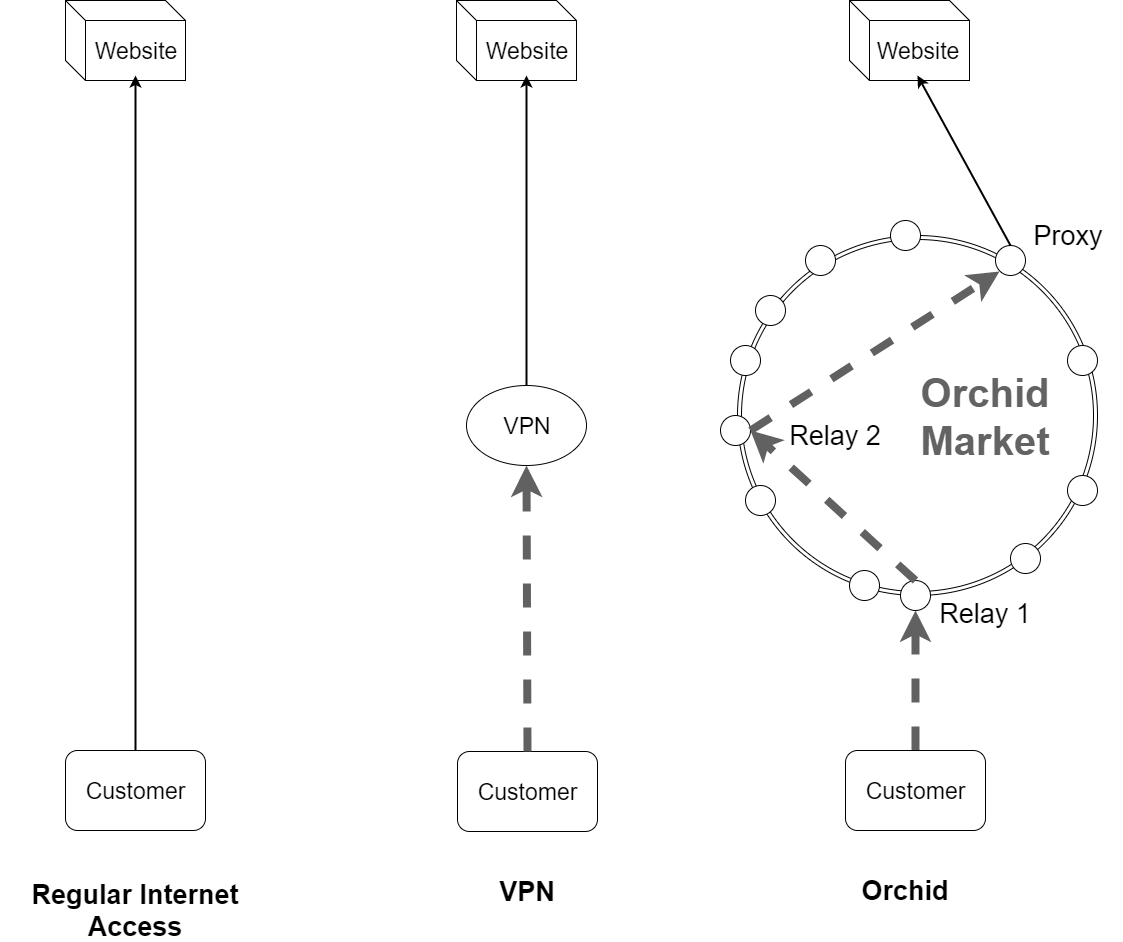
\includegraphics[width = 400pt]{overview}
  \caption{Direct connection, VPN connection, Orchid connection}
\end{figure}

Unlike more common methods for sending and receiving data from the
global Internet, proxy chains in \tOM{} naturally separate information
about the source of data from information about its destination; no
single bandwidth seller holds both pieces of information, or knows the
identity of bandwidth sellers who do. The rigid structure of \tOM{}
further supports this separation of information by providing strong
resistance against \emph{collusion attacks} -- the ability of a group
of bandwidth sellers to overcome this separation of knowledge.

Unlike less common methods for sending and receiving data from the
global Internet, which do compartmentalize source and destination
knowledge, \tOM{} provides \emph{fixed rate relaying} to prevent
traffic analysis, and an incentive for participation not related to
the hiding or discovery of information: payment in tokens.

Before we describe the details of the system, we will briefly review
the core problems it solves, and the general solutions we have chosen
for our system's foundation.

\subsection{The \emph{Traffic Analysis} Problem}

\textbf{Problem Statement:} Imagine you are in a cafeteria full of
mathematicians and wish to send a message to your friend across the
room without anyone else knowing that fact. You have not already
negotiated a message passing protocol, so all implementation details
must be publicly stated to everyone the room. What can be done?

A particularly elegant solution to this problem, proposed by Chaum in
1981\cite{chaum-mix}, is to have every person act as both a relay and
a recipient. In this scheme, participants prepare encrypted messages
which are the digital equivalent of ``envelopes containing envelopes''
-- to send a message to Alice, you would compute

$$Enc(``To Bob'' || Enc(``To Alice'' || Enc(message, Alice), Bob), Carol)$$

and send that message to Carol, who decrypts it and sends it to Bob,
who decrypts it and sends it to Alice. To prevent traffic analysis
everyone sends a fixed number of messages every cycle.  To handle
return addresses, we can have Bob and Carol remember a unique
message identifier and send messages back along the chain.

Of particular importance to systems using the above method is the
possibility of a \emph{Collusion}. If Bob and Carol cooperate they can
potentially determine who sent a given message, and to whom it was
sent.

\subsection{The \emph{Sybil} Problem}

The above cafeteria problem statement used physical bodies to
prevent \emph{Sybil Attacks} -- situations in which one participant
might pretend to be an arbitrarily large number of
users. Unfortunately, in digital systems this approach cannot be used.

\textbf{Problem Statement:} How can we know that someone is ``real''
in a purely digital context?

A solution to this problem can be found in Hashcash\cite{CHORD}. If we
require those claiming to be ``real'' to expend computational
resources, we can put Sybil Attackers in a position where claims of
being an incredible number of network participants requires actually
possessing an incredible amount of computational resources.

\subsection{The \emph{Random Selection} Problem}

The above cafeteria problem statement assumed an easy method for
sending a message to every other user of the system (e.g., yelling across
the cafeteria). To implement a Chaumian mix which is maximally
resistant to \emph{Collusion Attacks}, we need to be able to select
randomly from those relays who are ``real.'' Naively this requires
being notified whenever someone joins or leaves the network.
Unfortunately, in real-world P2P networks, having every user maintain
such a list would result in an unacceptable amount of network traffic
($O(n^2)$ notifications.)

\textbf{Problem Statement:} How can we maintain a distributed list of
all currently ``real'' relays which minimizes networking overhead and
supports efficient random selection of peers?

A particularly elegant solution to this problem can be found in the
Chord\cite{CHORD} Distributed Hash Table (DHT). In this scheme, peers
are assigned unique addresses in a large space and then are connected
in such a way that lookups can be performed in $O(log(n))$ time. Adding
or removing a user only requires notifying $O(log(n))$ peers.

\subsection{System Overview}

The \Orchid{} Protocol is, at its core, a combination of the above
solutions. In our approach, peers are required to
produce \emph{Medallions} to demonstrate their ``realness'', and are
then organized into a distributed P2P network termed the \emph{\Orchid{} Market}. To
keep \tOM{} participants honest, every peer checks the correctness of
its neighbor's behavior. Customers then use \tOM{} to select random
peers for Chaumian message forwarding. To incentivize participation,
we have Customers pay Relays on a per-forwarded-byte basis.

This is a simple idea, but of course the devil is in the details. The
system is to be fully decentralized, fully autonomous, fully
anonymous, and is to handle payments. Much of this design document is
therefore centered on preventing attacks on customer security, the system's performance, and the system's economic soundness. Although attack analysis is important, and will take up
much of our time, it is ultimately no more than a necessary conceit to
the context in which the market is to operate; if you find yourself
``lost in the woods'' we hope you will use the preceding exposition as
your north star -- the system's design details are all toward
realizing a real-world solution to the above trio of problems.
